
\tikzset{%
  % Specifications for style of nodes:
         base/.style = {rectangle, rounded corners, draw = black, minimum width=2.5cm, minimum height=1cm, fill=orange!15, font=\ttfamily},
}

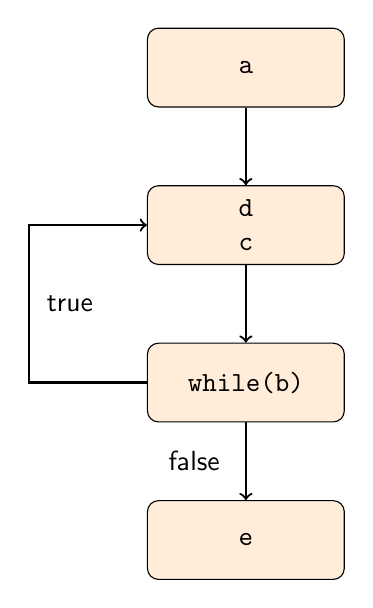
\begin{tikzpicture}[node distance=2cm, every node/.style={fill=white, font=\sffamily}, align=center]
    % Draw nodes
    \node (start)       [base]                        {a};
    \node (do)          [base, below of = start]      {d \\ c};
    \node (while)       [base, below of = do]         {while(b)};
    \node (end)         [base, below of = while]      {e};

    % Draw arrows
    \draw[->,thick]           (start) -- (do);
    \draw[->,thick]           (do) -- (while);
    \draw[->,thick]           (while) -- node[left=0.2cm, midway] {false} (end);

    \draw[->,thick]           (while.west) -- ++(-1.5,0) -- node[right= 0.1cm,midway]{true} ++(0,2) -- ++(1.5,0) (do);
\end{tikzpicture}
